\begin{wrapfigure}{R}{0.2\textwidth}
  \centering
  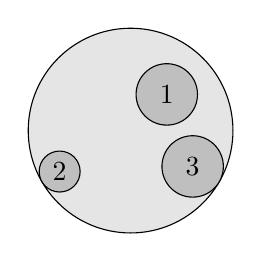
\begin{tikzpicture}[scale=1.3]
    \coordinate (a) at (45:0.5);
    \coordinate (b) at (210:0.8);
    \coordinate (c) at (-30:0.7);
    \filldraw [fill = gray!20] (0,0) circle (1);
    \filldraw [fill = gray!50] (a) circle (0.3) node {1};
    \filldraw [fill = gray!50] (b) circle (0.2) node {2};
    \filldraw [fill = gray!50] (c) circle (0.3) node {3};
  \end{tikzpicture}
\end{wrapfigure}
